\chapter{LITERATURE RESEARCH}

\paragraph\
This section explains the background research for the project. It gives a brief introduction about the services, architectures, and similar works done.

\section {\acs{ML}/\acs{AI} based Information Retrieval Services}
\paragraph\
This section gives a brief description of a few of the major service providers being tested in this project.

\subsection{\acs{IBM} Watson}
\paragraph\
\acs{IBM} Watson was named after \acs{IBM}'s founder Thomas J Watson. It was initially developed to hold human-like conversations in the natural language used by humans\cite{redefineibm}. However, it has grown way beyond just making conversations to analyzing hidden patterns and insights from not only structured but even unstructured data. \acs{IBM} Watson provides several products and services:
\begin{itemize}
    \item \acs{AI} assistance
    \item Data (Watson Studio\cite{urlIBMStudio}, Watson Machine Learning\cite{urlIBMMachineLearning}, Watson Knowledge Catalog\cite{urlIBMKowledgeCatalog})
    \item Knowledge
    \item Vision
    \item Speed
    \item Language
    \item Empathy
\end{itemize}

This thesis focuses on Watson \ac{NLU} \cite{watsonnlu}, which is a cloud-based service provided by \acs{IBM} that uses natural language processing and machine learning algorithms to analyze unstructured data such as text and provide insights. Some of the machine learning algorithms used by Watson \acs{NLU} include:

\begin{itemize}
    \item \ac{NER}: This algorithm identifies and extracts named entities such as people, organizations, and locations from the text.
    \item Sentiment analysis: This algorithm determines the emotional tone of a piece of text, whether it is positive, negative, or neutral.
    \item Concept tagging: This algorithm identifies concepts or topics present in a piece of text and assigns them to predefined categories.
    \item Emotion detection: This algorithm analyzes text to determine the emotions expressed by the writer, such as joy, sadness, anger, and fear.
    \item Relation extraction: This algorithm identifies and extracts relationships between entities in text, such as the relationship between a person and a company they work for.
    \item Content classification: This algorithm categorizes text into predefined categories based on its content, such as news, sports, or politics.
    \item Summarization: This algorithm generates a summary of a longer piece of text, highlighting the most important information.
    \item Language detection: This algorithm identifies the language of a piece of text, which can be useful for multilingual analysis.
\end{itemize}

These are just a few examples of the machine learning algorithms offered by Watson \acs{NLU}. 

\subsection{Microsoft Azure Cognitive Services}
Microsoft Azure Cognitive Services helps users to analyze, interpret, and search the datasets with a wide range of \acs{API}s provided. These \acs{API}s help in processing human language, sentiments, emotions, physical characteristics, audio, and more. 
Microsoft Cognitive Services\cite{azureCogOverview} \cite{del2018introducing} provides several services which can be categorized as below:
\begin{itemize}
    \item Vision
    \item Knowledge
    \item Language
    \item Speech
    \item Search
\end{itemize}

Microsoft Cognitive Services contains \acs{ML} algorithms in the form of simple-to-use \acs{REST} \acs{API}s and also has them available as \acs{SDK}s for a few languages\cite{azureCogServices}. Azure Cognitive Service for Language\cite{urlAzureCogLangOverview} provides \ac{NLP} features to understand and analyze text. With the help of Language Studio, users can use these service features without having to code. \ac{NER}, \ac{PII}, language detection, Sentiment analysis and opinion mining, summarization, key phrase extraction, entity linking, and question answering are some of the available \acs{NLP} features. \cite{urlAzureCogLangNLPfeatures} provides a detailed table for users to refer to be able to decide which feature to use for their applications based on their requirements. A few features are customizable too, where the user can train an \acs{AI} model to specifically fit their data using tools provided; and rest of them are pre-configured, meaning the user cannot change the \acs{AI} models being used by the feature. Figure \ref{azureNLPfeatures} gives a small glimpse of this table of features.

\begin {figure}[ht]
\centering
\adjustbox{frame}{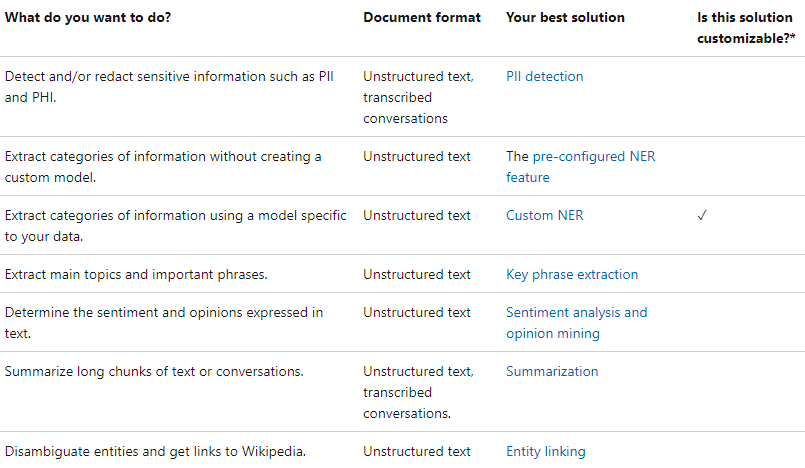
\includegraphics[scale=0.785]{images/Chapter2/Azure_NLP_features.png}}
\caption{Which Language service features to choose for your application}
\label{azureNLPfeatures}
\end {figure}

\subsection{Amazon Textract}
Amazon Textract \cite{urlAmazonTextract}\cite{archivedTextract} is \acs{ML} based service used to extract text, handwritten data, key-value pairs from scanned documents, tables, and forms automatically. This \acs{ML} service not only performs \ac{OCR} but also understands and extracts the data from \acs{pdf}s, images without manual effort. The document processing can be automated, and the extracted information can be utilized as required for further analysis. It provides an option for synchronous processing which would be useful to process a single-page document to get a faster response with low latency. Asynchronous processing option would be better when used for multi-page documents and high latency is not required \cite{archivedTextract}.

It currently claims to support the extraction of text from printed and handwritten invoices and receipts in the English language. However, it supports other languages like German, French, Spanish, Italian, and Portuguese along with English for text extraction from printed text, forms, and tables\cite{amazonLang}. Alfresco\cite{alfresco} is a free highly scalable content management platform. They provide one of the services named 'Intelligent Document Recognition Services, in which it uses the \acs{ML} and \acs{AI} from \ac{AWS} like
\begin{itemize}
    \item Amazon Textract\cite{urlAmazonTextract}
    \item Amazon Comprehend\cite{amazonComprehend}
    \item Amazon Rekognition\cite{amazonRekognition}
\end{itemize}to discover important insights from large volume of business content\cite{alfrescoAI}.

\subsection{Google Cloud}
Article \cite{kozlenko2021machine} states that Google Cloud Natural Language uses \acs{ML} techniques to extract information and meaning from unstructured text. Information like sentiment, mention of names, and locations can be extracted. They also provide syntax analysis along with entity and sentiment analysis with the help of pre-trained machine learning models. 
The book on Google Cloud Platform Services \cite{Bisong2019} mentions the various cloud services offered by Google Cloud \acs{AI} to its users. Figure \ref{gcaiservices} \cite{Bisong2019} shows the Google Cloud \acs{AI} services like 
\begin{itemize}
    \item Cloud Machine Learning Services (train and deploy machine learning models)
    \item Vision \acs{API} (classify/segment images)
    \item Speech \acs{API} (transcribe audio to text)
    \item Natural Language \acs{API} (extract/analyze text from documents)
    \item Translate \acs{API} (translate from one language to another)
\end{itemize}
\begin {figure}[h!h]
\centering
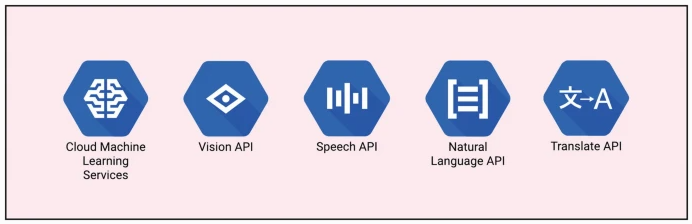
\includegraphics[scale=0.85]{images/Chapter2/google_cloud_ai_services.png}
\caption{Google Cloud \acs{AI} services}
\label{gcaiservices}
\end {figure}
This thesis focuses on Cloud Natural Language service as it aims to evaluate the information retrieval/extraction capabilities of the service provider. The features offered by Google Cloud Natural Language \acs{API} are sentiment analysis, entity recognition, entity sentiment analysis, and text classification \cite{gcdocs2}.

\section{Architectures}

\paragraph\
This section gives information about each of their architecture models based on the author's interpretation of the research.

\subsection{\acs{IBM} Watson \acs{NLU}}
\acs{IBM} Watson Studio provides a collaborative and integrated environment for data scientists, developers, and domain experts to work together on building and deploying \acs{AI} models. The architecture is composed of several components that work together to enable users to create, manage, and deploy machine learning models.

\begin {figure}[ht]
\centering
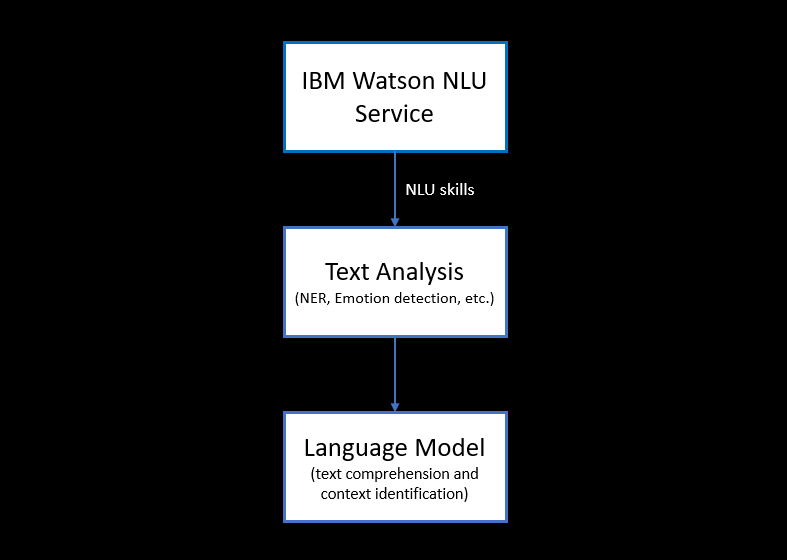
\includegraphics[scale=0.708]{images/Chapter2/IBM_arch3.png}
\caption{\acs{IBM} Watson \acs{NLU}}
\label{IBM_arch}
\end {figure}

Figure \ref{IBM_arch} depicts a very simple version of the \acs{IBM} Watson \acs{NLU} architecture. 
The IBM Watson \acs{NLU} service, which is in charge of supplying natural language understanding skills, is the main element of this design. It receives text as input and uses trained models to carry out a variety of text analysis tasks.

Text analysis, which comprises operations like entity recognition, sentiment analysis, keyword extraction, and emotion detection, constitutes the initial layer of processing in the \acs{NLU} service. To extract important information from the text, this layer employs machine learning algorithms and methods for natural language processing.

The language model, which is the following layer, is in charge of comprehending the language and context of the incoming text. To locate concepts, connections, and meanings within the text, it makes use of language conventions, semantic analysis, and statistical models.

In general, the IBM Watson \acs{NLU} architecture enables programmers to include language comprehension and natural language processing capabilities into their applications and to make use of text analysis and language processing methods to extract knowledge from unstructured textual input.

\subsection{Microsoft Azure Cognitive Services}

\begin {figure}[ht]
\centering
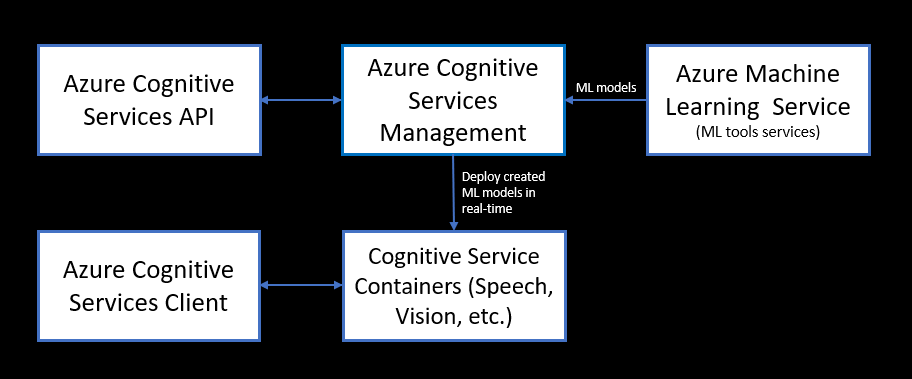
\includegraphics[scale=0.696]{images/Chapter2/Azure_arch.png}
\caption{Azure Cognitive Services}
\label{Azure_arch}
\end {figure}

Figure \ref{Azure_arch} illustrates how Azure Cognitive Services provides a collection of pre-built \acs{API}s and tools for developers to build intelligent applications with minimal machine learning expertise. The architecture is composed of several components that work together to enable users to leverage \acs{AI} and machine learning capabilities.

At the heart of the architecture is the Azure Cognitive Services Management layer, which provides access to pre-built \acs{AI} models and tools for speech recognition, natural language processing, computer vision, and other tasks. These services are accessed through the Azure Cognitive Services \acs{API}, which provides a unified interface for accessing the underlying \acs{AI} models. The Azure Cognitive Services \acs{API}  component provides the actual \acs{API}s that developers can use to access the cognitive services, while the Azure Cognitive Services Management component provides the management \acs{API}s for managing and monitoring the cognitive services.

Azure Machine Learning Service provides a suite of machine learning tools and services for building, training, and deploying models in the cloud or at the edge. Azure Machine Learning Service communicates with Azure Cognitive Services Management for authorization and management of Cognitive Services used in the Machine Learning Service. Azure Cognitive Services Management component interacts with the Azure Machine Learning Service, allowing users to deploy custom machine learning models created in the Azure Machine Learning Service to the Azure Cognitive Services containers for real-time inference.

The Azure Cognitive Services Client provides a simple way for developers to interact with the \acs{API}s and integrate them into their applications. The Cognitive Services Containers provide a way to run Cognitive Services on-premises or in other cloud environments.

Overall, the architecture of Azure Cognitive Services is designed to provide developers with a low-barrier entry for leveraging machine learning capabilities in their applications. By providing pre-built \acs{API}s and tools, Azure Cognitive Services enables developers to quickly and easily integrate intelligent features into their applications without the need for extensive machine learning expertise.


\subsection{Amazon Textract}

The architecture diagram in Figure \ref{Amazon_arch} \cite{amazonTextractArch} for \acs{AWS} Textract gives a high-level overview of the various components involved in the Textract service. Textract uses machine learning and \ac{OCR} to extract text and data from scanned documents.

\begin {figure}[ht]
\centering
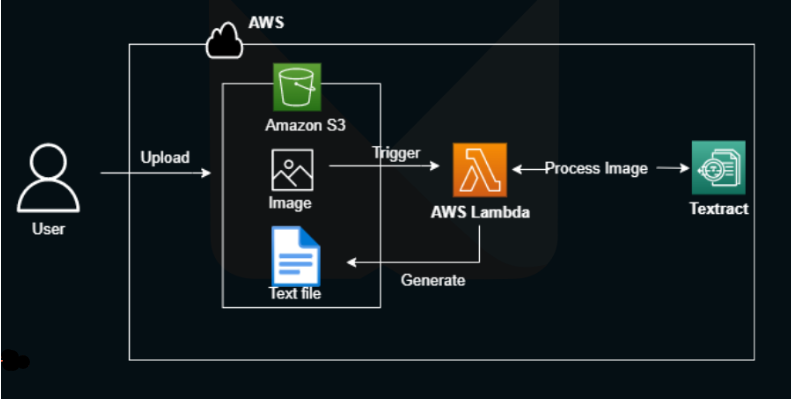
\includegraphics[scale=0.8]{images/Chapter2/Amazon_arch.png}
\caption{Amazon Textract}
\label{Amazon_arch}
\end {figure}

The architecture consists of the following components:
\begin{itemize}
    \item Input: The Textract service can accept input in various formats, such as image files (\acs{jpeg}, \acs{png}) or \acs{pdf} files.
    \item Amazon S3: Before being processed, the input files are stored in an S3 bucket, which is a highly scalable storage service provided by \acs{AWS}.
    \item \acs{AWS} Lambda: A server-less compute service that automatically runs code in response to events. \acs{AWS} Lambda is used to trigger the Textract service to process the input files.
    \item Amazon Textract: The machine learning service that performs \acs{OCR} and text extraction on the input files. Textract can automatically detect and extract text, tables, and other structured data from scanned documents. It claims \cite{urlAmazonTextract} to have higher capabilities than the average \acs{OCR} system.  It can extract information like names, birth dates, and social security numbers from the images and \acs{pdf} files that are stored in the S3 buckets. 
\end{itemize}

\acs{AWS} provides a database service Amazon DynamoDB. This is used to store the output of the Textract service, including the extracted text and metadata. \acs{AWS} also provides Amazon Comprehend, an \acs{NLP} service that analyzes text and extracts insights from it, such as sentiment analysis or entity recognition.

Overall, the architecture of \acs{AWS} Textract is designed to provide an efficient way to extract text and data from scanned documents. By leveraging machine learning and \acs{OCR}, Textract can automatically process documents and extract structured data that can be used for various purposes, such as data analysis or database population.

\subsection{Google Cloud Natural Language}

The Google Cloud Natural Language service is the core element of this system. It provides the user with natural language processing features that takes text as input and performs language analysis tasks using the Text analysis layer and provides output. The task of processing the incoming text and extracting valuable information including entity recognition, sentiment analysis, syntax analysis, and content classification is done by the Text Analysis layer. It analyzes the text and offers insights using machine learning models and language understanding techniques.

The Google Cloud Natural Language API allows developers to include advanced text analysis features offered by Google's natural language processing algorithms in their applications.

This is a brief overview of the architecture, emphasizing the key elements and data flow within the Google Cloud Natural Language. The final implementation would have additional components to make it fully functional and enable users to include language processing ability as part of their applications.


\section{Similar and Related Works}

\paragraph\
This section describes the similar and related works (three theses and one case study) done which have provided inspiration and reference for this thesis. 

\begin{itemize}
    \item Three data-analysis related studies were conducted in the thesis \cite{raji2018digital} by Raji et al. The third study involved performing predictive analysis using the machine Learning services in Microsoft Azure and \acs{IBM} Watson to examine their performance. In \cite{raji2018digital}, it was found that Azure performed better than \acs{IBM} Watson when evaluated on how well they performed and how user-friendly they were. Raji et al. chose Azure and \acs{IBM} machine learning services because of the add-and-drop feature. This feature enables the users to execute tasks on these services without the need for the user to have deep knowledge of machine learning or expert programming skills. Azure allows the user to freely choose from its wide set of services to use them alone or combined depending on the requirements of the task. \acs{IBM} also provides a similar feature to its users to use various services to achieve their goals. In this study\cite{raji2018digital}, predictive analysis was performed on both Azure and \acs{IBM} using three different datasets from Kaggle\cite{kaggle} and \acs{UCI} machine learning repository \cite{uciml}.
    The algorithms used to test the performance were Decision Trees, Logistic Regression, and Artificial Neural Networks. They tested each of the datasets with each of the three algorithms on both platforms. As both tools offered free initial trials, they were able to test the tools for ease of use, flexibility, and real-time predictions and chose the Azure platform to build the predictive model for the study. The sample of results for one of the datasets can be seen in Figure \ref{similar_work_results}.
    \begin {figure}[ht]
    \centering
    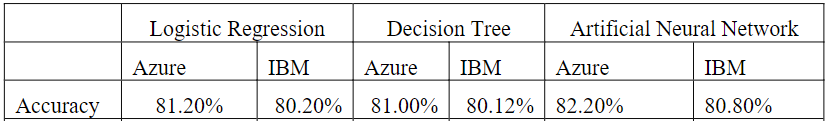
\includegraphics[scale=0.77]{images/Chapter2/similar_work.png}
    \caption{Model Evaluation for Default Credit Card Payment Dataset}
    \label{similar_work_results}
    \end {figure}
    After training, their predictive model built in Azure gave them a Mean Absolute Error of 11\%. The lesser the value, the more accurate the model's predictions are. In conclusion of \cite{raji2018digital}, it is stated that \acs{IBM} and Azure were initially compared to check the performance to build a predictive model. And based on the faster data analysis performance by Azure when compared to \acs{IBM}, they decided to build their predictive analysis model in the Azure cloud platform. 
    
    \item In \cite{rollino2022automating} we can see that Amazon Textract and Amazon Open Search were used to extract financial information from financial reports. Thesis \cite{rollino2022automating} was checking the possibility of automating the process of extracting financial data from European companies. In \cite{rollino2022automating}, two systems were created, first to collect the financial reports and the second to extract data from these reports. Rollino et al. used web-scrapping to achieve the first system and Textract, Open Search from \acs{AWS} for the second. They configured Textract to discard the characters identified with less than 90\% confidence and the tool worked so well that not even a single character was discarded. The extracted information was sent to Amazon Comprehend through the lambda function. Output was then displayed as key-value pairs with financial keywords and financial numbers respectively that were successfully extracted by Amazon Open Search. Figure \ref{similar_work_arch} shows a simplified overview of how they used \acs{AWS} services to extract financial information from the reports.
    \begin {figure}[ht]
    \centering
    \adjustbox{frame}{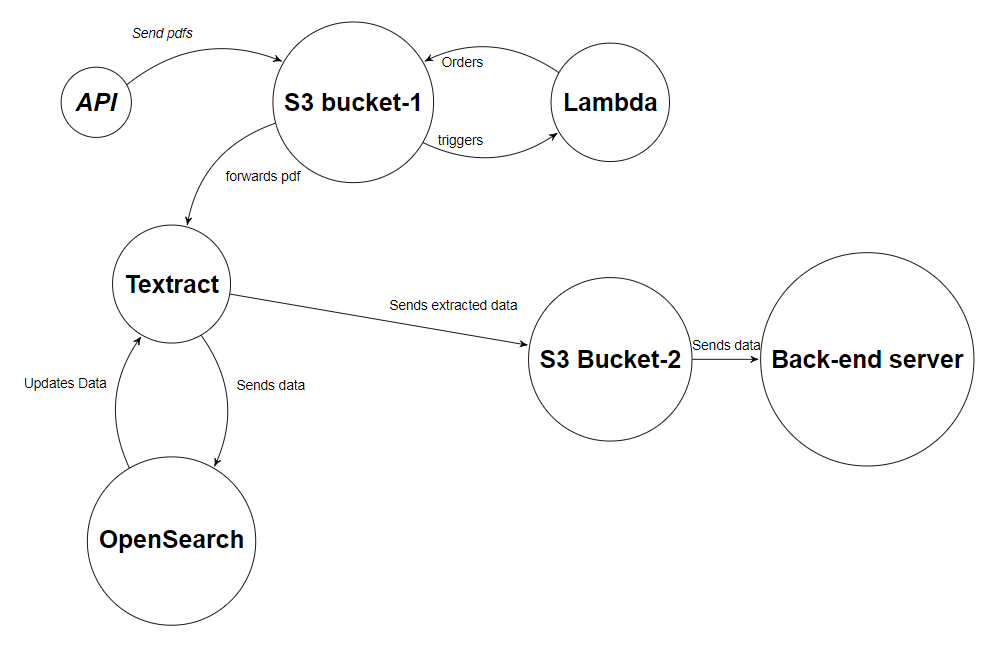
\includegraphics[width=0.95\textwidth]{images/Chapter2/similar_work_diag.png}}
    \caption{Simplified overview of data processing using Amazon Web Services}
    \label{similar_work_arch}
    \end {figure}
    It was found at the end that extraction of data was possible from the reports however they faced the bottleneck in the stage to obtain these financial reports as the task at hand was too complex due to the differences in designs of reports used by every European company. There was no 'one fits all' solution to collect the reports and hence it was left for the future scope to solve the bottleneck of collecting financial reports to supply to the tool to extract required data points.

    \item A Swedish thesis report \cite{eriksson2018granskning} mentions that cloud services is one of the highly progressive and fast growing fields. Many companies like \acs{IBM}, Google, Amazon, and Microsoft offer various comparable and similar services and features in a competitive spirit. \cite{eriksson2018granskning} aimed at examining the applicability of cloud services majorly \acs{IBM} Watson services, and checking the possibility of making an automated thesis examiner using \acs{IBM} Watson. Most of the \acs{IBM} Watson services were evaluated but there wasn't sufficient time to explore the Machine learning service thoroughly. In \cite{eriksson2018granskning} it was found that although there were quite a lot of applications for Watson Web Services, they were unable to find a service suitable to build an automated thesis examiner which was the goal of \cite{eriksson2018granskning}. Though the goal was not achieved, \cite{eriksson2018granskning} was still a work to refer for the Watson Services applications.

    \item In the case study \cite{2017honda}, Honda, a Japanese origin, now global automobile manufacturing company used \acs{IBM} Watson's cognitive solutions to understand and extract useful information from large unstructured quality-related data (from various social platforms like Twitter, Reddit, Facebook, etc.) as part of its Quality Assurance efforts. Little et al. state that "Use of the \acs{IBM} solution by Honda shows how cognitive systems and technologies can improve and augment human capabilities as well as improve overall analysis and decision making. Organizations should be evaluating cognitive technologies in general and text analytics, in particular, to determine where, how, and when these can be applied to business processes, thereby improving performance, quality, and productivity." Honda had two main challenges to be addressed. The first is a faster identification of issues as the parts are distributed globally, a faulty part would arise a global challenge and would need to be addressed as early as possible. Hence, the need to identify and correct the issue quickly was the first challenge. The Second was to gather customer feedback from all different regions and classify them in a way to identify if the issue was already addressed in any one of the regions. As all of this was being done manually, it was consuming a lot of time and Honda needed this process to be automated to get faster results. Hence, Honda worked with \acs{IBM} and implemented a cognitive solution to extract and classify incoming feedback and provide a visual dashboard representation highlighting key factors as required by each unit. Honda also initially evaluated SAS \cite{sas} and \acs{IBM} with a sample dataset to compare the results from both offers. While evaluating, they found that \acs{IBM}'s tool was easier to use and hence worked with \acs{IBM} to create a solution for its challenges. They used \acs{IBM} Watson Explorer Advanced Edition which included advanced analytic capabilities to extract domain-specific information and identify patterns, trends, and relations from unstructured content. 
    This cognitive system used text analytics and helped Honda achieve not only a faster response rate to customer feedback but also a greater understanding of customer issues. By using the \acs{IBM} solution, Honda was able to interpret and classify incoming customer feedback 80\% faster. \acs{IBM} combined its solution with \acs{IBM} Cognos Business Intelligence\cite{cognosBI} graphs and reports which helped in summarizing and categorizing issues along with highlighting the identified trends on the dashboard.
    At the time, Honda was also exploring \acs{IBM} Watson Developer Cloud Services to further automate the classification process using \acs{ML} and \acs{AI}. The case study ended with a note stating that cognitive solutions should be considered as enhancements to human efforts and as complete replacements.
\end{itemize}